\documentclass[a4paper, 14pt]{extarticle}

\usepackage{amsmath}
\usepackage{amssymb}
\usepackage{amsthm}
\usepackage{commath}
\usepackage[margin=0.5in]{geometry}
% \usepackage{lexend}
\usepackage{microtype}
\usepackage{parskip}
\usepackage{tikz}
\usepackage{tikz-cd}
\usepackage{tkz-euclide}
\usepackage{xparse}

\usetikzlibrary{calc,angles,quotes, positioning, shapes.geometric}

\theoremstyle{definition}
\newtheorem{dfn}{Definition}
\newtheorem{clm}{Claim}
\newtheorem{asn}{Assertion}
\newtheorem{thm}{Theorem}
\newtheorem{prb}{Problem}
\newtheorem{ans}{Answer}
\newtheorem{lm}{Lemma}
\newtheorem{rmk}{Remark}
\newtheorem{crl}{Corollary}
\newtheorem{ex}{Exercise}
\newtheorem{xmp}{Example}

\newcommand{\titleheader}[1]{\begin{centering}
\begin{LARGE}
\textbf{#1}
\end{LARGE}\\
\hrulefill

\vspace{-1.25\baselineskip}
\hrulefill
\end{centering}\\\\}

\def\changemargin#1#2{\list{}{\rightmargin#2\leftmargin#1}\item[]}
\let\endchangemargin=\endlist

\NewDocumentEnvironment{smrg}{}{\begin{changemargin}{0.5cm}{0.5cm}}{\end{changemargin}}

\NewDocumentEnvironment{SWP}{m m}
{%
  \vspace{-.9cm}%
  \begin{changemargin}{0.5cm}{0.5cm}%
  \noindent#1~#2
  \par
  \textbf{Proof.} 
}
{%
  \qed
  \end{changemargin}
}

\NewDocumentEnvironment{SNP}{m}
{%
  \vspace{-.9cm}%
  \begin{changemargin}{0.5cm}{0.5cm}%
  \noindent#1
}
{%
  \end{changemargin}
}

\newcommand{\bb}[1]{\mathbb{#1}}
\newcommand{\st}{\space \mid \space}
\newcommand{\union}[1]{\displaystyle\mathop{\cup}\limits_{#1}}
\newcommand{\intersect}[1]{\displaystyle\mathop{\cap}\limits_{#1}}
\newcommand{\paran}[1]{\left ( {#1} \right )}
\newcommand{\contra}{$\rightarrow\!\leftarrow$}
\newcommand{\kvec}[2]{({#1}_1 \dots {#1}_{#2})}
\newcommand{\pf}{\textbf{Proof.} }

\newcommand{\AnswerSection}{
    \newpage
    \section*{Answers to Exercises}
    \textit{The following are brief solutions or hints. You are encouraged to review the exercises before checking the answers.}
}
\begin{document}
\titleheader{Power Series}
\textbf{Prereqs} RA-19
\begin{SNP}{\dfn}A series of the form
$$
\sum\limits_{n = 0}^{\infty}a_n(x - a)^n
$$
is called a \emph{power series around} $a$, or simply a power series.
\end{SNP}

The number $a$ is colloquially called the ``center'' of the power series.

The convergence or divergence of a power series clearly depends on the value of $x$. As an example, consider
$$
\sum\limits_{n = 0}^{\infty}x^n
$$
We know a priori this is the geometric sum and it converges to $\frac{1}{1 - x}$ iff $\abs{x} < 1$. i.e., if $x \in (-1, 1)$ then our series converges, otherwise it doesn't converge, and therefore depending on the value of $x$.

Let's consider another series,
$$
\sum\limits_{n = 0}^{\infty}n!x^n
$$
Using the ratio test, $\abs{\frac{a_{n + 1}}{a_n}} = (n + 1)\cdot \abs x \to \infty$, except when $x = 0$. Thus the series only converges for $x = 0$ and for no other $x$.

Finally consider the series
$$
\sum\limits_{n = 0}^{\infty}\dfrac{x^n}{n!}
$$
Using the ratio test again, $\abs{\frac{a_{n + 1}}{a_n}} = \frac{\abs x}{n + 1} \to 0$ for every $x$. Thus the series converges for every $x \in \bb R$.

So we have made a few observations. A power series around $a$ always converges for $x = a$. Now except for the extreme cases where the series only converges for $x = a$ or converges on the entire real line, it appears that the series converges inside some open interval around $a$ and doesn't converge outside of it.

Refer to the geometric series example, in which a power series around $a = 0$ converges in $(-1, 1)$ and diverges outside of it, which is an interval of \textit{radius} $1$ around $a$.

It so happens that this is precisely how power series behave.
\begin{SWP}{\lm}{Consider a power series
$$f(x) := \sum a_n (x - a)^n$$
\begin{enumerate}\item If $f(x_0)$ converges, and $x_1$ is such that $\abs{x_1 - a} < \abs{x_0 - a}$ then $f(x_1)$ converges absolutely.\item If $f(x_0)$ doesn't converge, and $x_1$ is such that $\abs{x_1 - a} > \abs{x_0 - a}$ then $f(x_1)$ doesn't converge.\end{enumerate}}Suppose $\sum a_n (x_0 - a)^n$ converges, thus $\exists$ $M > 0$ such that $\abs{a_n (x_0 - a)^n} \leq M$ for every $n$ $(\ast)$. Now consider
\begin{align*}
\abs{a_n (x_1 - a)^n} &= \abs{a_n}\abs{x_1 - a}^n\\
					  &= \abs{\dfrac{x_1 - a}{x_0 - a}}^n \cdot \abs{a_n}\abs{x_0 - a}^n\\
					  &\leq M\cdot q^n
\end{align*}
where $q < 1$, hence the series
$$
\sum \abs{a_n}\cdot \abs{x_1 - a}^n
$$
is bounded above by a convergent geometric series therefore converges. As a consequence, the series
$$
\sum a_n\cdot (x - a)^n
$$
also converges.

Now suppose $\sum a_n (x_0 - a)^n$ does not converge and $x_1$ is such that $\abs{x_1 - a} > \abs{x_0 - a}$. If at all the series $\sum a_n (x_1 - a)^n$ converges, by the previous part of the theorem, $\sum a_n (x_0 - a)^n$ will converge. Contradiction. Thus $\sum a_n (x_1 - a)^n$ does not converge.
\end{SWP}

Where I've used the result $(\ast)$ -- that a convergent series is uniformly bounded. Allow me to make this precise.
\begin{SNP}{\ex}Suppose $\sum a_n$ converges. Show that for some $M > 0$, $\abs{a_n} < M$ for every $n$.
\end{SNP}

Let me make the lemma a little more clear. Suppose for some power series around a point $a$, I know of its convergence and divergence at two points.
\begin{center}
\begin{tikzpicture}[scale=1]
  % Number line
  \draw[->] (-5.5,0) -- (5.5,0) node[right] {$x$};
  % Ticks at -y, 0, x
  \foreach \t in {-4,0,2}
    \draw (\t,0.1) -- (\t,-0.1);
  % Labels
  \node[below] at (0,0) {$a$};
  \node[above] at (2,0) {$a+x$};
  \node[above] at (-4,0) {$a-y$};
  % Points
  \fill[red]   (2,0) circle (3pt);
  \fill[blue]  (-4,0) circle (3pt);
\end{tikzpicture}\\
Suppose a power series centered at $a$ converges at $a + x$ and doesn't converge at $a-y$
\end{center}
We just saw that for points closer to $a$ than $x$, the series necessarily converges, and for those further away than $-y$, it necessarily diverges. Let's have a look.
\begin{center}
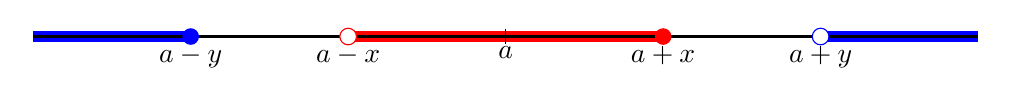
\begin{tikzpicture}[scale=1]
  % 1) colored “divergence” regions (blue)
  \draw[blue, line width=4pt] (-6,0) -- (-4,0);
  \draw[blue, line width=4pt] (4,0)  -- (6,0);
  % 2) colored “convergence” region (red)
  \draw[red,  line width=4pt] (-2,0) -- (2,0);

  % underlying number line
  \draw[thick] (-6,0) -- (6,0);

  % ticks
  \foreach \t in {-4,-2,0,2,4}
    \draw (\t,0.1) -- (\t,-0.1);

  % labels
  \node[below] at (0,0)  {$a$};
  \node[below] at (2,0)  {$a+x$};
  \node[below] at (-2,0) {$a-x$};
  \node[below] at (4,0)  {$a+y$};
  \node[below] at (-4,0) {$a-y$};

  % filled/open circles
  \fill[red]         (2,0) circle (3pt);      % known converge
  \draw[red, fill=white]   (-2,0) circle (3pt); % inconclusive at -x

  \fill[blue]        (-4,0) circle (3pt);     % known diverge
  \draw[blue, fill=white]  (4,0)  circle (3pt); % open at +y
\end{tikzpicture}\\
The power series doesn't converge in the blue region, and converges in the red region
\end{center}
This is what the lemma is saying. The existence of a singular blue or red point directly gives you the existence of blue and red ``regions'' where the behavior of the power series is known.

Observe -- the behavior at $a + x$ is not enough to conclude the behavior at $a - x$. Similarly the behavior at $a - y$ is not enough to conclude the behavior at $a + y$.

The sharp eyed will notice that a power series \textit{must} fall into one of two categories -- a) converges or b) doesn't converge for every fixed $x$. i.e., the sum $\sum a_n(x - a)^n$ either converges or it doesn't, no third thing can happen.

All in all, the red and blue regions should \textit{completely} cover the number line. The lemma has also given us something special -- the red region most definitely exists (every power series around $a$ converges at $x = a$) -- but also, it must be \textit{sandwiched} between the blue region.

Formally, this is what we're getting at.
\begin{SWP}{\thm}{(Trichotomy) Consider the power series
$$
\sum a_nx^n
$$Then the series either only converges at $x = 0$ and nowhere else, converges on the entire number line, or there exists a unique $r > 0$ such that the series absolutely converges when $\abs{x} < r$ and doesn't converge when $\abs{x} > r$.}We only need to show that if the first two don't happen then the third necessarily does.

Suppose the series converges at some point $x_c \neq 0$ and doesn't converge at some other point $x_d$. We know from the lemma that $\abs{x_c} \leq \abs{x_d}$. Consider the set
$$
S := \{r \in \bb R_{\geq 0} \st \text{the series converges for both $-r$ and $r$}\}
$$
We know that $\frac{\abs{x_c}}{2}$ is in $S$ (since the series converges for $x_c$ it converges for both $\frac{x_c}{2}$ and $-\frac{x_c}{2}$) and $\abs{x_d}$ is an upper bound of $S$ (by the lemma the series does not converge at any $x_0$ with $\abs{x_0} > \abs{x_d}$).

Let $\alpha$ be the least upper bound of $S$. We will show $\alpha$ is the required $r$.

Let $x_1$ be such that $\abs{x_1} < \alpha$. Since $\alpha$ is the lub of $S$, $\abs{x_1}$ is NOT an upper bound of $S$ and thus there is some $r' \in S$ with $\abs{x_1} < r' < \alpha$. But then the series converges for $r'$ and $\abs{x_1} < r'$ therefore the series converges for $x_1$.

Now suppose $x_2$ is such that $\abs{x_2} > \alpha$. By whatever theorem you'd like to invoke there is some $r'$ such that $\abs{x_2} > r' > \alpha$. If the series converges for $x_2$, it must converge for $r'$ and $\alpha$ fails to be an upper bound of $S$. Thus the series does not converge for $x_2$.
\end{SWP}
This unique $r$ is called the \emph{radius of convergence} of the power series.

Replacing $x$ with $x - a$ keeps all the above arguments intact, allowing us to neatly sum up the following result.
\begin{SNP}{\crl}A power series
$$
\sum a_n(x - a)^n
$$
\begin{enumerate}
	\item either converges only at $x = a$
	\item or converges for all values of $x$
	\item or converges on some interval $(a - r, a + r)$ and diverge outside it. The behavior at the boundary points $x = a - r$ and $x = a + r$ is \textbf{inconclusive} in this case and needs to be seperately investigated.
\end{enumerate}
\end{SNP}
\begin{SNP}{\xmp}Consider the power series $\sum\limits_{n = 1}^{\infty}\frac{x^n}{n}$. Using the root test, we get $\lim \abs{a_n}^{1/n} = \abs{x}$. So whenever $\abs{x} < 1$, the series converges, and whenever $\abs{x} > 1$, the series doesn't converge. Hence it converges for $x \in (0-1, 0+1)$ and doesn't converge outside of it.

What about when $\abs{x} = 1$? For $x = -1$, we recognise this as the famous series approximation of $\ln \frac 1 2$ (neat!). While for $x = 1$, we've already shown in RA-18 that the series diverges to $\infty$.

Therefore, it is critical that we investigate the boundaries properly. Indeed, the interval of convergence of the series is $[-1, 1)$.
\end{SNP}
Finally, I'd like you to look at this neat little trick to find the radius of convergence of a power series.
\begin{SNP}{\thm}Consider a power series$$\sum a_n(x - a)^n$$\begin{enumerate}
  \item If $\lim\limits_{n\to \infty}\abs{a_n}^{1/n} = L$, then the radius of convergence of the series is $\frac{1}{L}$, where if $L = \infty$ then the series only converges at $a$, and if $L = 0$ it converges everywhere.
  \item If $\lim\limits_{n\to \infty}\abs{\dfrac{a_{n + 1}}{a_n}} = L$ then the radius of convergence of the series is $\frac{1}{L}$, where if $L = \infty$ then the series only converges at $a$, and if $L = 0$ it converges everywhere.
\end{enumerate}
\end{SNP}
One can verify this by using the Trichotomy Theorem and the ratio and root tests for the power series.
\AnswerSection
\ans Suppose $\sum a_n$ converges, then the sequence of partial sums $S_n$ is bounded, i.e there is some $K > 0$ such that $\abs{S_n} < K$ for every $n$. Now $a_n = S_n - S_{n - 1}$ for $n > 1$ and $a_1 = S_1$. Thus,
\begin{align*}
\abs{a_n} \leq \abs{S_n} + \abs{S_{n - 1}} < 2K
\end{align*}
and thus $a_n$ is bounded.
\end{document}